\section{Introduction}

\begin{itemize}
    \item Interactive visualization of data
    \item Making the text transparent, with the possibility to highlight the data related to a specific sentence.
    \item Making sense of data-driven claims is hard, even if the evidence base (code/data) is open
    \item We see this in peer review, misinformation, retracted papers, …
\end{itemize}

\subsection{Self-Certifying Text}

\begin{itemize}
    \item Introduce basic idea, as complementary to transparent visualisations
\end{itemize}

\begin{figure}
    \centering
    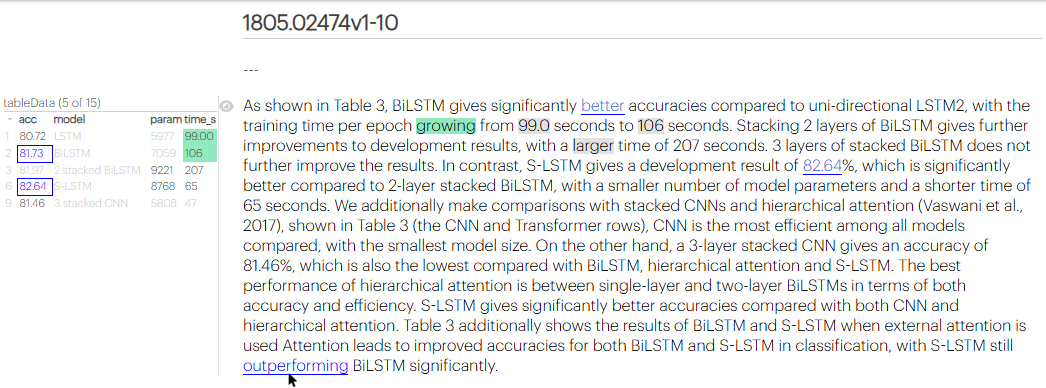
\includegraphics[width=\linewidth]{fig/scigen-mr-1906.02780-10.png}
    \caption{Website example with the generated expression from authoring assistant}\label{fig:scigen-example-website}
\end{figure}


\subsection{Use cases}
Two potential scenarios for this sort of technology:

\paragraph{Authoring transparent text.} Someone authoring content for an online article, wants to create text
linked to raw data (and derivative data such as charts or tabular summaries), so that the evidence base for
the claims made in the text can be explored \emph{in situ}, by interacting with the text.

\paragraph{Interpreting text after the fact.} Someone reading textual claims derived from open data (e.g. a
scientific paper or climate report), wants to retroactively link the text to queries over the available data
and gradually ``rationally reconstruct'' the relationship between the claims in the paper and the evidence
base. Perhaps just to aid their own comprehension, or to provide some kind of justified peer review.

\vspace{2mm}
\noindent Here we focus on the first one because the second one requires a certain amount of additional setup.

\subsubsection{Target idioms of natural language}

NLP aspect of the problem is potentially a big problem space in itself. We will restrict interest to certain
idiomatic uses of natural language in making/justifying scientific claims.
Examples \ref{tab:fluid_examples}

\begin{table}[!ht]
    \centering
    \footnotesize
    \renewcommand{\arraystretch}{1.1}
    \begin{tabular}{>{\raggedright\arraybackslash}p{2cm} >{\raggedright\arraybackslash}p{5cm} >{\raggedright\arraybackslash}p{6cm}}
        \toprule
        \textbf{Type}                & \textbf{Example} & \textbf{Generated Expression} \\
        \midrule
        \rowcolor{gray!20}
        \multicolumn{3}{>{\raggedright\arraybackslash}l}{\textbf{Quantitative expressions}} \\

        Numerical value
        & the training time per epoch growing from \hl{67} seconds to 106 seconds.
        &%check with v-space
        \vspace{-5pt}
        \begin{lstlisting}[language=Fluid,numbers=none]
(findWithKey' "model" "LSTM" tableData).time_s
        \end{lstlisting}
        \\
        Percentage &
        The Energy Sector accounts for total methane emissions of \hl{52.80\%} in 2030.
        &
        \vspace{-5pt}
        \begin{lstlisting}[language=Fluid,numbers=none]
(record.emissions /
 sum (map (fun x -> x.emissions)
          (getByYear year tableData))) * 100

        \end{lstlisting}  \\
        Rounding & ~                & ~                             \\
        Cardinals \& Multiplicative & ~                & ~                             \\
        \rowcolor{gray!20}
        \multicolumn{3}{>{\raggedright\arraybackslash}l}{\textbf{Aggregation}} \\
        Average
        & The average methane emissions for the year 2030 is \hl{13.51} &
        \vspace{-5pt}
        \begin{lstlisting}[language=Fluid,numbers=none]
(sumEmissions year tableData / length records)
        \end{lstlisting} \\
        Min/Max                          & The Energy Sector recorded its highest methane emissions in \hl{2030}             &
        \vspace{-5pt}
        \begin{lstlisting}[language=Fluid,numbers=none]
let maxEntry =
    maximumBy (fun x -> x.emissions)
              (filter
                (fun x -> x.type == "Energy Sector")
                tableData)
in maxEntry.year
        \end{lstlisting} \\                             \\
        Ranks &
        3-layer stacked CNN gives an accuracy of 81.46\%, which is the \hl{lowest} compared with BiLSTM, and S-LSTM  &
        \vspace{-5pt}
        \begin{lstlisting}[language=Fluid,numbers=none]
let pos =
  findIndex "model" "CNN"
    (insertionSort cmpTime tableData)
in rankLabel "lowest" pos
        \end{lstlisting} \\
        Total &
        The total methane emissions for the year 2030 is \hl{37.74} for Agriculture &
        \vspace{-5pt}
        \begin{lstlisting}[language=Fluid,numbers=none]
sumEmissions year tableData
        \end{lstlisting} \\
        Count*                       & ~                & ~                             \\
        \rowcolor{gray!20}
        \multicolumn{3}{>{\raggedright\arraybackslash}l}{\textbf{Trends}} \\

        Comparisons
        & The training time per epoch \hl{growing} from 67 seconds to 106 seconds. &
        \vspace{-5pt}
        \begin{lstlisting}[language=Fluid,numbers=none]
trendWord
 (findWithKey' "model" "BiLSTM" tableData).time_s
 (findWithKey' "model" "LSTM" tableData).time_s
 growShrink
        \end{lstlisting} \\
        Graded adjective*            & ~                & ~                             \\
        Reference to visual element*                            & ~                & ~                             \\
        \bottomrule
    \end{tabular}
    \caption{Example expressions generated by the Authoring Assistant, classified by type. In green, the expression is already tested.}
    \label{tab:fluid_examples}
    \renewcommand{\arraystretch}{1.0}
\end{table}
\subsection{Contributions}

\begin{itemize}
    \item Design and proof-of-concept implementation of AI-assisted workflow for authoring transparent text
    (\secref{authoring-workflow})
    \item Empirical evaluation of how effective current LLMs are at providing the ``AI-assisted'' part
\end{itemize}
